\documentclass[11pt,a4paper]{article}

\usepackage[T1]{fontenc}
\usepackage[utf8]{inputenc}
\usepackage{lmodern}
\usepackage[margin=2.5cm]{geometry}
\usepackage{microtype}
\usepackage{amsmath}
\usepackage{booktabs}
\usepackage{tabularx}
\usepackage{threeparttable}
\usepackage{multirow}
\usepackage{xcolor}
\usepackage{pgfplots}
\pgfplotsset{compat=1.18}
\usepackage[numbers,sort&compress]{natbib}
\usepackage[hidelinks]{hyperref}
\usepackage{enumitem}
\setlist{nosep,leftmargin=*}

\definecolor{gwin}{HTML}{1F4E79}
\definecolor{gloss}{HTML}{CC0000}
\definecolor{gnull}{HTML}{5F6368}

\newcommand{\pp}{\,pp}
\newcommand{\nb}[1]{NB\,#1}
\newcolumntype{Y}{>{\raggedright\arraybackslash}X}

\title{Where Do Knowledge Graphs Help LLM Agents?\\[2pt]
\large Nineteen Experiments, from Hand-Built Examples to Benchmarks with Thousands of Questions}

\author{Dimitar Trajanov\\
\small Faculty of Computer Science and Engineering, Ss.\ Cyril and Methodius University -- Skopje\\
\small \texttt{dimitar.trajanov@finki.ukim.mk}}

\date{Companion report to the 2nd SMASHING Workshop lecture\\ ``LLM-Based Agentic Systems and Knowledge Graphs'', October 2026}

\begin{document}
\maketitle

\begin{abstract}
Knowledge graphs are widely proposed as a remedy for the weaknesses of retrieval-augmented LLM agents: multi-hop
reasoning, questions about whole collections, facts that change over time, unverifiable query generation and
untrusted content. We test these claims in nineteen executable experiments. Ten smaller notebooks
(up to 300 questions, \texttt{gpt-4o-mini}) illustrate each claim; nine \emph{confidence runs} then re-test them on
public benchmarks with 115--4{,}072 questions each, stronger baselines and paired 95\% confidence intervals
(\texttt{gpt-6-luna} without reasoning, about 160{,}000 LLM calls, about \$29 in total). Graphs give large, reliable
gains when the answer depends on \emph{structure}: aggregates over typed records (+51\pp\ on templated helpdesk
questions), whole-collection questions (+19.8\pp\ of expected content), and multi-hop questions over relational data
(+57 to +67 Hits@1 at two and three hops on MetaQA, even with a graph the LLM extracted from text, which scored 11--24
points below the curated graph). Elsewhere gains are small or absent: +4.7 and +11.7 F1 on MuSiQue and
2WikiMultiHopQA; +1.0 and +2.7 points on GraphRAG-Bench with HippoRAG2-style ranking, and losses with a simpler graph
retriever; $-50$\pp\ on single-fact lookups; no gain on helpdesk questions written without the graph ($-8$\pp, not
reliable). Baselines that encode the same information in simpler form match the graph: document dates match a temporal
graph ($-0.2$\pp), and stating a schema's naming rules in the prompt recovers all but 2--5 points of an ontology
checker's +61.5\pp. GraphRAG's global search loses 30\pp\ on local questions, where its local search nearly matches
vector retrieval. These findings agree with recent RAG-versus-GraphRAG comparisons and extend them to agent memory,
query checking and guardrails. We conclude that graphs should be adopted per question type, against the strongest
cheap baseline; their robust value lies in structure, and rules enforced in code add a guarantee of zero violations
rather than a large gain in accuracy.
\end{abstract}

% =====================================================================================
\section{Introduction}

The combination of large language model (LLM) agents and knowledge graphs (KGs) is promoted for at least six
distinct purposes: (i) answering relational and multi-hop questions by traversal~\cite{yao2023react,sun2024thinkongraph};
(ii) answering questions about an entire corpus through community summaries (GraphRAG)~\cite{edge2024graphrag};
(iii) improving retrieval by graph-based ranking (HippoRAG)~\cite{gutierrez2024hipporag,gutierrez2025hipporag2};
(iv) maintaining long-term, time-aware agent memory~\cite{rasmussen2025zep};
(v) validating LLM-generated graph queries against an ontology~\cite{sequeda2023benchmark,allemang2024ontologies};
and (vi) enforcing provenance, workflow and plan rules as guardrails~\cite{debenedetti2025camel,beurerkellner2025patterns}.
Recent controlled comparisons find that the benefit of graph retrieval depends strongly on the question type and
that plain retrieval remains better for single-hop, detail-oriented questions~\cite{han2025ragvsgraphrag,zhou2025unified,xiang2025graphragbench}.
These studies concentrate on retrieval and question answering; the other roles are usually evaluated in isolation,
against plain top-$k$ retrieval, or on small samples.

This report collects the results of nineteen notebooks written as companions to a lecture on agentic systems and
knowledge graphs. Notebooks 01--07 are instructional: small, realistic data sets on which each claim can be
observed and inspected. Notebooks 08--10 repeat three comparisons on public benchmarks. Notebooks 11--19 are
confidence runs designed to test each claim at scale: every one uses a public benchmark or a templated question set
large enough for narrow intervals, adds the strongest cheap baseline we could identify, and archives every LLM
request and response.

\paragraph{Contributions.}
\begin{itemize}
  \item One protocol applied to six roles of KGs in agentic systems---retrieval, sensemaking, temporal knowledge,
        memory, query generation and guardrails---with paired 95\% intervals for every headline difference
        (Sections~\ref{sec:structure}--\ref{sec:guardrails}). Prior comparisons cover mainly the first two.
  \item Baselines that give plain retrieval the same information in simpler form (document dates, the full
        conversation history, the schema's rules in the prompt, retry on error), which match or nearly match the
        graph in several cases, and stronger graph methods (HippoRAG2-style ranking, GraphRAG local search) where our
        first implementation lost (Section~\ref{sec:discussion}).
  \item A decision guide stating for which question types a graph is worth its indexing and per-query cost
        (Table~\ref{tab:verdict}).
\end{itemize}

% =====================================================================================
\section{Related Work}
\label{sec:related}

\paragraph{Graph-based retrieval.} Surveys organise graph RAG into graph construction, graph retrieval and
graph-augmented generation~\cite{peng2024survey,zhang2025survey,zhu2026survey}; representative systems include
GraphRAG~\cite{edge2024graphrag}, LightRAG~\cite{guo2024lightrag} and HippoRAG~\cite{gutierrez2024hipporag,gutierrez2025hipporag2}.
Several studies compare these systems with plain retrieval under one protocol. \citet{han2025ragvsgraphrag} find
that RAG is better on single-hop and detail-oriented questions and GraphRAG on multi-hop questions, and that
community-based global search often struggles on question answering. \citet{zhou2025unified} re-implement graph RAG
methods in a unified framework. \citet{xiang2025graphragbench} build GraphRAG-Bench with medical and novel corpora
and four question types and report gains mainly for complex reasoning and summarisation; a different benchmark of
the same name~\cite{xiao2025graphragbench} uses textbook questions. All GraphRAG-Bench results in this report refer
to the benchmark of \citet{xiang2025graphragbench}. \citet{zhuang2026linearrag} report that relation extraction can
introduce noise that lowers retrieval quality. Our notebooks~11, 14 and~16 re-test these claims; the rest of the
report extends the comparison beyond retrieval.

\paragraph{Agent memory.} Zep~\cite{rasmussen2025zep} and Mem0~\cite{chhikara2025mem0} store conversation facts in
a (temporal) graph. Benchmarks for long-term memory include LongMemEval~\cite{wu2025longmemeval},
LoCoMo~\cite{maharana2024locomo} and MemoryAgentBench~\cite{hu2026memoryagentbench}. Two published results bear
directly on our full-history baseline: long-context models lose 30--60\% accuracy on LongMemEval-S compared with
reading only the evidence sessions~\cite{wu2025longmemeval}, whereas on LoCoMo a full-context baseline (72.9) scores
above Mem0 with graph memory (68.4) and Zep (66.0)~\cite{chhikara2025mem0}; A-Mem~\cite{xu2025amem} links memory
notes without a fixed schema. More generally, \citet{li2024ragorlc} find that sufficiently capable long-context models
outperform RAG on average when the input fits in the context window, at a much higher token cost.

\paragraph{Time-aware knowledge.} Temporal question answering over text and knowledge graphs is surveyed
by \citet{piryani2025temporalqa}. HoH~\cite{ouyang2025hoh} measures the harm of outdated passages in retrieval; its
questions ask for the current value of a fact, which is the setting of our notebook~12, not questions about the state
of the world at a past time.

\paragraph{Queries over knowledge graphs.} \citet{sequeda2023benchmark} show that answering over a knowledge-graph
representation of an enterprise database raises LLM accuracy compared with SQL over the same data, and
\citet{allemang2024ontologies} add ontology-based query checks with LLM repair. Spider4SPARQL~\cite{kosten2023spider4sparql}
and Spider4SSC~\cite{vejvar2025spider4ssc,vejvar2026singlequery} translate Spider~\cite{yu2018spider} into SPARQL
(and, for Spider4SSC, Cypher).

\paragraph{Guardrails against prompt injection.} InjecAgent~\cite{zhan2024injecagent} and AgentDojo~\cite{debenedetti2024agentdojo}
benchmark indirect prompt injection in tool-using agents. CaMeL~\cite{debenedetti2025camel} extracts the control and
data flow of a task from the trusted user query before untrusted data is read and enforces security policies when
tools are called; \citet{beurerkellner2025patterns} describe related patterns such as plan-then-execute. Our plan
graph is a simplified instance of this idea: it restricts which tools may be called but, unlike CaMeL, does not
track data flow.

% =====================================================================================
\section{Methods Compared}
\label{sec:methods}

\paragraph{Vector retrieval (baseline).} Texts are embedded with \texttt{text-embedding-3-small}; for each
question the $k$ most similar texts ($k$ between 3 and 20, stated per experiment) are given to the LLM with a
fixed answer prompt. Wherever possible the baseline receives a comparable amount of context to the graph method.

\paragraph{Graph agent.} An LLM in a ReAct loop~\cite{yao2023react} calls read-only tools that look up nodes,
follow typed edges, filter and count. Tools cannot modify data.

\paragraph{HippoRAG-style graph retrieval.} The LLM extracts subject--relation--object triples (OpenIE) from
every passage; entities with embedding similarity $\geq 0.9$ are linked by synonym edges; personalised
PageRank~\cite{haveliwala2002ppr} seeded at the question's entities ranks passages~\cite{gutierrez2025hipporag2}.

\paragraph{GraphRAG community summaries.} Entities and relations are extracted from every chunk and clustered with
Louvain~\cite{blondel2008louvain}, split recursively to at most 25 entities. Each community is summarised in
advance; a question is answered map-reduce style over all summaries~\cite{edge2024graphrag}.

\paragraph{Bi-temporal graph memory.} Facts extracted from conversations or documents carry validity intervals;
a contradicting fact closes the earlier one (\texttt{invalid\_at}) rather than deleting it~\cite{rasmussen2025zep}.
Retrieval returns current facts with dates and source turns.

\paragraph{Ontology-checked queries.} A deterministic checker tests each class and property of an LLM-written
SPARQL query against the ontology (vocabulary, direction, domain/range, grounding of named entities). Violations
are explained to the LLM, which may repair the query up to three times~\cite{allemang2024ontologies}.

\paragraph{Graph guardrails.} \emph{Provenance filtering} admits content only if its origin in the graph is
trusted. A \emph{workflow graph} blocks an action whose prerequisite steps are not complete. A \emph{plan graph}
is fixed by the LLM before any untrusted tool output is read; code refuses every tool call outside the plan
(a plan-then-execute pattern~\cite{beurerkellner2025patterns,debenedetti2025camel}).

% =====================================================================================
\section{Experimental Setup}
\label{sec:setup}

\paragraph{Data.} Table~\ref{tab:data} lists the nineteen experiments. Instructional data include a synthetic
IT-helpdesk graph (Aura; 23 tickets, 57 comments, 246 typed links), the ServiceNow incident event log
(20{,}769 incidents)~\cite{uci2018incident}, 183 generated (synthetic) hospital-software support tickets (PlanetCare), 58 synthetic security runbooks with
version metadata, and a $\tau^2$-bench telecom workflow~\cite{barres2025tau2}. Public benchmarks are
MetaQA~\cite{zhang2018metaqa}, MuSiQue~\cite{trivedi2022musique}, 2WikiMultiHopQA~\cite{ho2020twowiki},
HoH~\cite{ouyang2025hoh}, InjecAgent~\cite{zhan2024injecagent} with the AgentDojo attack
template~\cite{debenedetti2024agentdojo}, GraphRAG-Bench~\cite{xiang2025graphragbench},
LongMemEval~\cite{wu2025longmemeval}, LoCoMo~\cite{maharana2024locomo}, BenchmarkQED~\cite{benchmarkqed2025} and
Spider4SSC~\cite{vejvar2025spider4ssc,yu2018spider}. For \nb{11} we use the 1{,}000 development questions per benchmark
released with HippoRAG~2~\cite{gutierrez2025hipporag2}; each benchmark's passages form one shared pool (11{,}656
paragraphs for MuSiQue, 6{,}119 for 2WikiMultiHopQA), so every question is answered among the distractors of all
others. For \nb{17} we take the full Spider4SSC development split (608 questions over 20 databases), drop the 36
questions of one database whose 45\,MB graph is too large for our in-memory SPARQL engine, and drop 9 questions whose
gold query fails to execute, leaving 563 questions over 19 graphs. All \nb{17} systems receive the full schema,
including each graph's namespace, in the prompt. For \nb{19} we use the 18{,}127 WikiMovies articles (first
paragraphs) from which MetaQA's knowledge base was built~\cite{miller2016kvmemnn}, and sample 300 MetaQA test
questions per hop (seed 7) whose topic entity is a film with an article, so this sample differs from \nb{08}'s.

\paragraph{Models.} Notebooks 01--10 use \texttt{gpt-4o-mini}; notebooks 11--19 use \texttt{gpt-6-luna} (the API version
available in October 2026) with reasoning disabled; results with reasoning enabled, or with other models, may
differ. All calls use temperature 0 and seed 7; because API outputs are not guaranteed to be
deterministic even with a fixed seed, reproducibility rests on the response cache described below. Confidence runs are executed through the OpenAI
Batch API; agent loops run in lock-step, one batch per step. Stages added after review whose batch jobs stalled for
hours, including the agent loops of \nb{19}, were sent through the standard API with identical request bodies.

\paragraph{Scoring.} Exact match, F1 or execution accuracy wherever a gold answer can be computed; LLM judges
only for open-ended answers, with the benchmark's own judge prompt where one exists and both presentation orders
for pairwise comparisons. The judge is the same model as the answering model (\texttt{gpt-4o-mini} in 01--10,
\texttt{gpt-6-luna} in 11--19) and receives answers without method labels (pairwise comparisons as ``answer 1'' and ``answer 2'' in both
orders). Answers can still differ in style---GraphRAG answers, for example, cite community reports---so the judge may
be able to infer the method.

\paragraph{Statistics.} Single accuracies carry Wilson intervals~\cite{wilson1927}; differences between methods
on the same questions carry paired bootstrap intervals~\cite{efron1993bootstrap}. A difference is called
\emph{reliable} when its 95\% interval excludes zero. Intervals are not adjusted for multiple comparisons. As a
check, we widened each of the 26 headline intervals in Figure~\ref{fig:forest} by the Bonferroni factor
$z_{0.05/52}/z_{0.025}\approx 1.58$ (normal approximation): 23 keep their classification, while three reliable
differences become \emph{borderline}: the +16\pp\ gain on verified fixes (\nb{18}), and the $-1.5$-point loss of the
simple graph retriever and the +1.0-point gain of the HippoRAG2-style retriever on GraphRAG-Bench medical (\nb{14}). Subgroup results in Tables~\ref{tab:multihop}--\ref{tab:memory} should be read
with the same caution.

\paragraph{Reproducibility.} Every LLM request is cached under a hash of its full body, so each notebook replays
its results without API calls when the cache is present. All 159{,}932 logged requests and responses of the confidence runs (and 945 of small
test runs), and the raw input and output files of all 70 batch jobs, are archived with a manifest. Clustering was made independent of
Python hash randomisation and verified under two seeds.

\begin{table}[t]
\centering
\small
\caption{The nineteen experiments. \nb{} = notebook; ``Re-tests'' names the instructional notebook whose claim a
confidence run repeats at scale.}
\label{tab:data}
\begin{tabularx}{\textwidth}{@{}lYlr@{}}
\toprule
NB & Claim examined and data & Re-tests & Questions \\
\midrule
01 & Graph agent vs.\ vector retrieval on a helpdesk graph (Aura) & -- & 22 \\
02 & ReAct traversal for multi-hop questions (ServiceNow incidents) & -- & 10 \\
03 & LLM graph construction: entity resolution, extraction, validation (hospital tickets) & -- & -- \\
04 & Bi-temporal retrieval against replaced and conflicting runbooks & -- & 56 \\
05 & Provenance and workflow guardrails (Aura, $\tau^2$-bench telecom) & -- & 10 + 10 runs \\
06 & GraphRAG for whole-collection questions (hospital tickets) & -- & 3 \\
07 & Ontology-checked SPARQL generation (Aura as RDF) & -- & 15 \\
08 & Multi-hop traversal on MetaQA & -- & 300 \\
09 & HippoRAG-style retrieval on GraphRAG-Bench (medical sample) & -- & 180 \\
10 & Bi-temporal memory on LongMemEval-S (sample) & -- & 108 \\
\midrule
11 & HippoRAG-style retrieval on MuSiQue and 2WikiMultiHopQA & 08 & 2{,}000 \\
12 & Temporal graph vs.\ retrieval with and without dates on HoH & 04 & 500 \\
13 & Plan-graph gate against indirect prompt injection (InjecAgent) & 05 & 3{,}162 \\
14 & GraphRAG-Bench in full, medical and novel domains & 09 & 4{,}072 \\
15 & Graph memory vs.\ vector vs.\ full history (LongMemEval-S, LoCoMo) & 10 & 2{,}040 \\
16 & GraphRAG on BenchmarkQED podcast transcripts, global and local & 06 & 100 \\
17 & Ontology checker vs.\ retry baseline on Spider4SSC & 07 & 563 \\
18 & Helpdesk, graph agent vs.\ vector retrieval: templates, and questions written without the graph & 01 & 156 + 115 \\
19 & Graph agent over a curated vs.\ an LLM-extracted graph on MetaQA & 08 & 900 \\
\bottomrule
\end{tabularx}
\end{table}

% =====================================================================================
\section{Results}

Figure~\ref{fig:forest} summarises every headline difference of the confidence runs; the following subsections
report each group of experiments.

\begin{figure}[p]
\centering
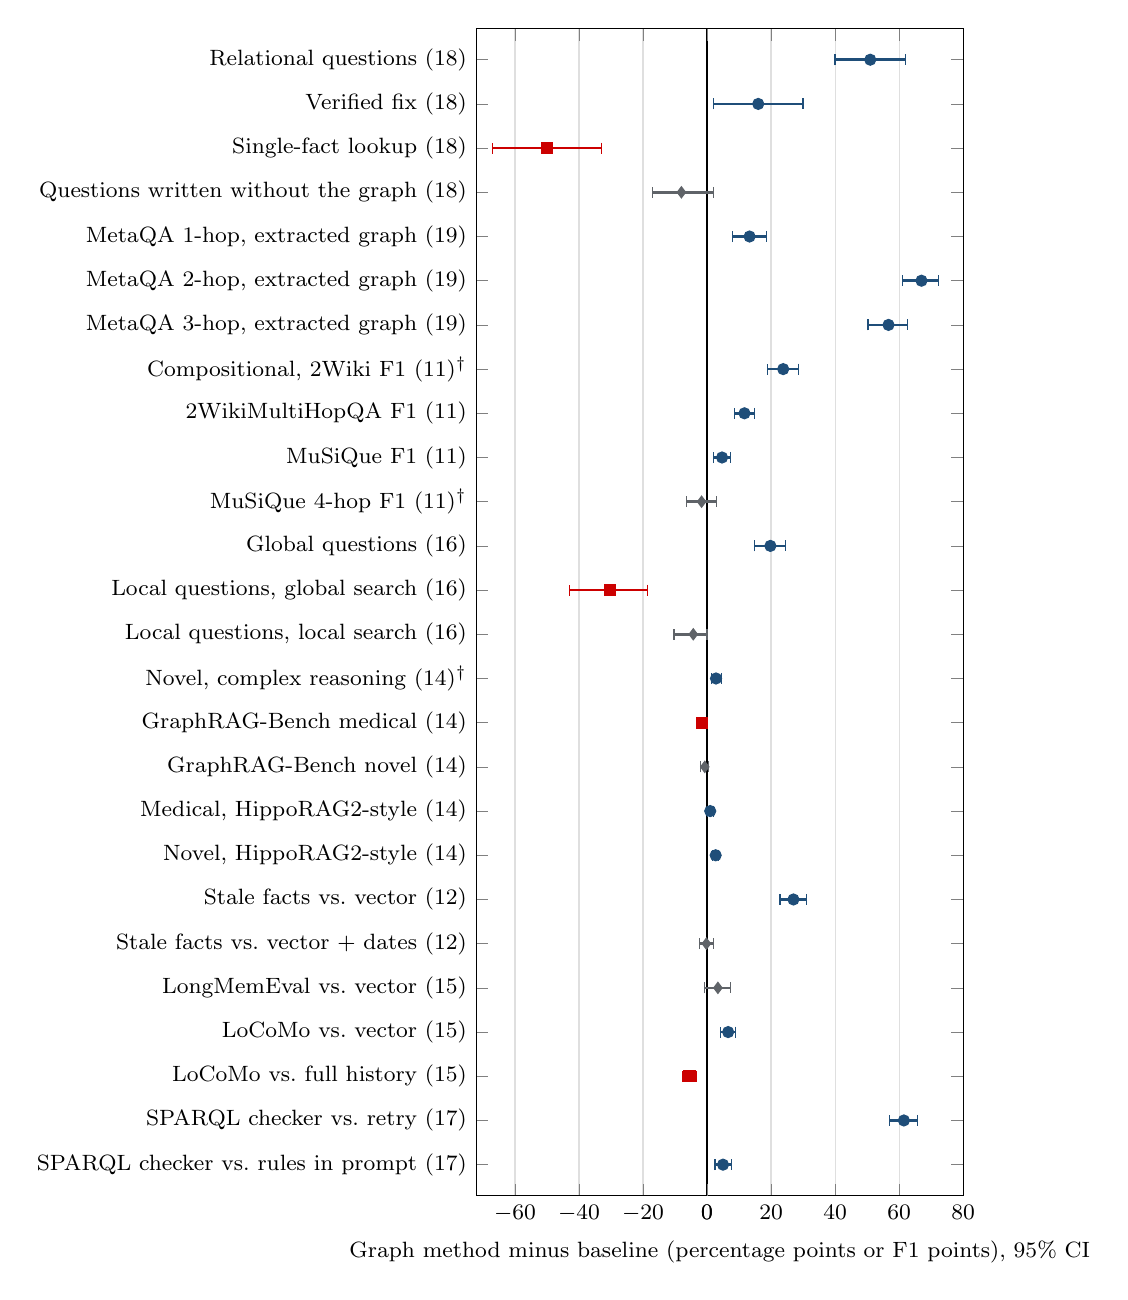
\begin{tikzpicture}
\begin{axis}[
  width=0.64\textwidth, height=16.4cm,
  xmin=-72, xmax=80,
  ymin=0.3, ymax=26.7, y dir=reverse,
  ytick={1,...,26},
  yticklabels={
    {Relational questions (18)},
    {Verified fix (18)},
    {Single-fact lookup (18)},
    {Questions written without the graph (18)},
    {MetaQA 1-hop, extracted graph (19)},
    {MetaQA 2-hop, extracted graph (19)},
    {MetaQA 3-hop, extracted graph (19)},
    {Compositional, 2Wiki F1 (11)$^\dagger$},
    {2WikiMultiHopQA F1 (11)},
    {MuSiQue F1 (11)},
    {MuSiQue 4-hop F1 (11)$^\dagger$},
    {Global questions (16)},
    {Local questions, global search (16)},
    {Local questions, local search (16)},
    {Novel, complex reasoning (14)$^\dagger$},
    {GraphRAG-Bench medical (14)},
    {GraphRAG-Bench novel (14)},
    {Medical, HippoRAG2-style (14)},
    {Novel, HippoRAG2-style (14)},
    {Stale facts vs.\ vector (12)},
    {Stale facts vs.\ vector + dates (12)},
    {LongMemEval vs.\ vector (15)},
    {LoCoMo vs.\ vector (15)},
    {LoCoMo vs.\ full history (15)},
    {SPARQL checker vs.\ retry (17)},
    {SPARQL checker vs.\ rules in prompt (17)}},
  yticklabel style={font=\footnotesize},
  xticklabel style={font=\footnotesize},
  xlabel={Graph method minus baseline (percentage points or F1 points), 95\% CI},
  xlabel style={font=\footnotesize},
  xmajorgrids, grid style={gray!25},
  extra x ticks={0}, extra x tick style={grid style={black, thick}},
  error bars/error bar style={line width=0.9pt},
]
\addplot+[only marks, mark=*, color=gwin, mark options={fill=gwin},
  error bars/.cd, x dir=both, x explicit]
  coordinates {
    (51,1) += (11,0) -= (11,0)
    (16,2) += (14,0) -= (14,0)
    (13.3,5) += (5.4,0) -= (5.3,0)
    (67.0,6) += (5.3,0) -= (6.0,0)
    (56.7,7) += (6.0,0) -= (6.4,0)
    (23.8,8) += (4.7,0) -= (4.8,0)
    (11.7,9) += (3.1,0) -= (3.1,0)
    (4.7,10) += (2.7,0) -= (2.6,0)
    (19.8,12) += (4.8,0) -= (4.9,0)
    (2.8,15) += (1.6,0) -= (1.5,0)
    (1.0,18) += (0.9,0) -= (0.9,0)
    (2.7,19) += (1.0,0) -= (0.9,0)
    (27.0,20) += (4.2,0) -= (4.2,0)
    (6.6,23) += (2.4,0) -= (2.4,0)
    (61.5,25) += (4.2,0) -= (4.5,0)
    (5.0,26) += (2.6,0) -= (2.5,0)
  };
\addplot+[only marks, mark=square*, color=gloss, mark options={fill=gloss},
  error bars/.cd, x dir=both, x explicit]
  coordinates {
    (-50,3) += (17,0) -= (17,0)
    (-30.3,13) += (11.6,0) -= (12.7,0)
    (-1.5,16) += (1.1,0) -= (1.0,0)
    (-5.5,24) += (2.1,0) -= (2.1,0)
  };
\addplot+[only marks, mark=diamond*, color=gnull, mark options={fill=gnull},
  error bars/.cd, x dir=both, x explicit]
  coordinates {
    (-8,4) += (10,0) -= (9,0)
    (-1.7,11) += (4.6,0) -= (4.6,0)
    (-4.3,14) += (4.3,0) -= (6.0,0)
    (-0.7,17) += (1.2,0) -= (1.2,0)
    (-0.2,21) += (2.2,0) -= (2.2,0)
    (3.4,22) += (4.0,0) -= (4.2,0)
  };
\end{axis}
\end{tikzpicture}
\caption{Headline differences of the confidence runs (notebook in brackets). Blue circles: reliable gains for
the graph method; red squares: reliable losses; grey diamonds: intervals including zero. Units are percentage
points of accuracy or Hits@1 (18, 19), of expected content (16) or of answer correctness (14), and F1 points (11).
$^\dagger$One subgroup out of four to eight, chosen for illustration; Tables~\ref{tab:multihop}--\ref{tab:grb} list
all subgroups, and of the eight GraphRAG-Bench cells only this one favours the simple graph retriever. The helpdesk
families and question sets (18), MetaQA hops (19) and the global and local question sets (16) are designed groups,
all shown. Rows added after review: 4, 5--7, 14, 18--19 and 26.}
\label{fig:forest}
\end{figure}

% -------------------------------------------------------------------------------------
\subsection{Structural and Multi-Hop Questions}
\label{sec:structure}

\paragraph{Small samples.} On the Aura helpdesk (\nb{01}), vector retrieval and a graph agent were similar on
simple lookups (5/5 vs.\ 4/5), but the agent found the confirmed fix in 11/11 cases against 7/11, and answered
5/6 relational questions against 1/6. On ServiceNow incidents (\nb{02}), a ReAct agent answered 8 of 10 multi-hop
questions against 1 of 10 for top-10 retrieval, at 6.5 times the tokens (4{,}194 vs.\ 646 per question). On
MetaQA (\nb{08}), Hits@1 was 91\% vs.\ 99\% for one hop, 39\% vs.\ 97\% for two hops and 36\% vs.\ 80\% for
three hops, with token ratios of 1.7, 3.0 and 6.6.

\paragraph{At scale.} Table~\ref{tab:multihop} reports \nb{11}. When the graph is extracted from text by the LLM
(190{,}347 triples), HippoRAG-style retrieval improves F1 by +4.7 [+2.1, +7.4] on MuSiQue and +11.7
[+8.6, +14.8] on 2WikiMultiHopQA. The gain is concentrated in compositional questions (+23.8) and in two-hop
MuSiQue questions (+7.9); it vanishes at three and four hops and reverses on comparison questions, which name
both entities explicitly ($-5.0$ [$-9.3$, $-0.7$]). Retrieval recall explains much of the pattern: the graph
raised recall@5 of gold passages from 70.6\% to 84.4\% on 2Wiki but only from 55.3\% to 58.4\% on MuSiQue.

\nb{19} separates the effect of extraction from that of the benchmark by staying on MetaQA. The LLM extracted facts
in MetaQA's nine relations from the 18{,}127 WikiMovies articles (146{,}006 triples). It recovered 71\% of the curated
triples about the sampled topic films: 96--99\% of directors, actors and release years, 78\% of writers, 90\% of
genres, but only 7\% of tags and no IMDb ratings, which the articles rarely state. The same graph agent then answered
300 questions per hop over the curated and over the extracted graph, against vector retrieval of the ten most similar
articles (Table~\ref{tab:metaqa}). The extracted graph kept most of the advantage: +13.3, +67.0 and +56.7 Hits@1 over
vector retrieval at one, two and three hops, with the curated graph a further 11--24 points higher. Vector retrieval
fails at two and three hops (9\% and 12\%) because the answers are attributes of other films, which no article about
the topic film contains. The agents used 1{,}900--2{,}200 tokens per question against 1{,}600 for vector retrieval;
extraction cost \$0.92 for all articles.

\nb{18} repeats \nb{01} with 156 templated questions whose answers are computed from the graph
(Table~\ref{tab:helpdesk}). The structural split holds with tight intervals: the graph agent wins relational
questions by +51\pp\ and verified fixes by +16\pp, but loses lookups by $-50$\pp, a larger loss than the small
sample suggested. Because the gold answers are computed from the same graph the agent queries, and the templates
ask what the agent's tools compute (counts, filters, joins), this design favours the graph agent.
We therefore added a second question set written without the graph: an LLM that saw only the 90 texts indexed
for vector retrieval wrote 119 questions with answers, of which 115 were confirmed by an independent full-context
reading. None of its 58 multi-record questions matches an existing template; they ask for narrative details
spread over several tickets rather than for counts. On this set the advantage disappears: graph minus vector is
$-14$\pp\ [$-28$, $-3$] on lookups, $-4$ [$-25$, +18] on fixes, $-7$ [$-21$, +9] on multi-record questions and
$-8$ [$-17$, +2] overall. The relational gain therefore holds for questions whose answer is an aggregate over typed
records, not for multi-record questions in general. The writer and validator read text, so this set in turn favours
text-shaped questions; together the two sets bound the effect from both sides.

\begin{table}[t]
\centering
\small
\caption{Multi-hop question answering over text (\nb{11}): token F1, top-5 passages, 1{,}000 questions per
benchmark. Differences with paired 95\% bootstrap intervals.}
\label{tab:multihop}
\begin{tabular}{@{}llrrrl@{}}
\toprule
Benchmark & Group & $n$ & Vector & Graph & Graph $-$ vector \\
\midrule
\multirow{4}{*}{MuSiQue}
 & 2-hop & 518 & 43.7 & 51.6 & \textbf{+7.9} [+4.2, +11.6] \\
 & 3-hop & 316 & 36.6 & 39.4 & +2.9 [$-2.1$, +7.9] \\
 & 4-hop & 166 & 24.3 & 22.6 & $-1.7$ [$-6.3$, +2.9] \\
 & All & 1{,}000 & 38.2 & 43.0 & \textbf{+4.7} [+2.1, +7.4] \\
\midrule
\multirow{5}{*}{2WikiMultiHopQA}
 & Compositional & 413 & 23.8 & 47.6 & \textbf{+23.8} [+19.0, +28.5] \\
 & Inference & 108 & 47.2 & 62.9 & \textbf{+15.7} [+7.2, +23.9] \\
 & Bridge comparison & 235 & 61.9 & 67.6 & +5.7 [$-2.2$, +13.3] \\
 & Comparison & 244 & 89.2 & 84.2 & $\mathbf{-5.0}$ [$-9.3$, $-0.7$] \\
 & All & 1{,}000 & 51.2 & 62.9 & \textbf{+11.7} [+8.6, +14.8] \\
\bottomrule
\end{tabular}
\end{table}

\begin{table}[t]
\centering
\small
\caption{MetaQA with a curated and an LLM-extracted graph (\nb{19}, 300 questions per hop): Hits@1 with Wilson
intervals; differences in points with paired 95\% bootstrap intervals. Both graphs are queried by the same agent.}
\label{tab:metaqa}
\footnotesize\setlength{\tabcolsep}{3.5pt}
\begin{tabular}{@{}llllll@{}}
\toprule
Hops & Vector top-10 & Curated graph & Extracted graph & Extracted $-$ vector & Curated $-$ extracted \\
\midrule
1 & 60\% [55, 66] & 85\% [81, 89] & 74\% [68, 78] & \textbf{+13.3} [+8.0, +18.7] & \textbf{+11.3} [+7.3, +15.7] \\
2 & 9\% [6, 13] & 100\% [99, 100] & 76\% [71, 80] & \textbf{+67.0} [+61.0, +72.3] & \textbf{+24.0} [+19.3, +29.0] \\
3 & 12\% [9, 17] & 93\% [90, 95] & 69\% [64, 74] & \textbf{+56.7} [+50.3, +62.7] & \textbf{+24.0} [+18.7, +29.3] \\
\bottomrule
\end{tabular}
\end{table}

\begin{table}[t]
\centering
\small
\caption{Helpdesk questions by family (\nb{18}): accuracy with Wilson intervals. Top: 156 templated questions
with gold answers computed from the graph. Bottom: 115 questions written by an LLM from the ticket texts only and
confirmed by an independent reading; all are judged against the written answer.}
\label{tab:helpdesk}
\footnotesize\setlength{\tabcolsep}{4pt}
\begin{tabular}{@{}lrlll@{}}
\toprule
Family & $n$ & Vector top-8 & Graph agent & Graph $-$ vector \\
\midrule
\multicolumn{5}{@{}l}{\emph{Templated questions, gold from the graph}} \\
Single-fact lookup & 30 & 97\% [83, 99] & 47\% [30, 64] & $\mathbf{-50}$ [$-67$, $-33$] \\
Verified fix & 44 & 73\% [58, 84] & 89\% [76, 95] & \textbf{+16} [+2, +30] \\
Relational (counts, filters) & 82 & 46\% [36, 57] & 98\% [92, 99] & \textbf{+51} [+40, +62] \\
All & 156 & 63\% [56, 71] & 85\% [79, 90] & \textbf{+22} [+12, +31] \\
\midrule
\multicolumn{5}{@{}l}{\emph{Questions written from the texts, without the graph}} \\
Single-fact lookup & 29 & 100\% [88, 100] & 86\% [69, 95] & $\mathbf{-14}$ [$-28$, $-3$] \\
Problem and fix & 28 & 50\% [33, 67] & 46\% [30, 64] & $-4$ [$-25$, +18] \\
Multi-record & 58 & 67\% [54, 78] & 60\% [47, 72] & $-7$ [$-21$, +9] \\
All & 115 & 71\% [62, 79] & 63\% [54, 72] & $-8$ [$-17$, +2] \\
\bottomrule
\end{tabular}
\end{table}

% -------------------------------------------------------------------------------------
\subsection{Corpus-Wide Sensemaking and Graph-Based Retrieval}
\label{sec:sensemaking}

\paragraph{Small samples.} On 183 hospital tickets (\nb{06}), GraphRAG answers were judged more comprehensive in
6 of 6 comparisons, mentioned 10 of 10 hospitals against 5, and cited 43 real ticket IDs against 9, at 10.6 times
the tokens per question. On a 180-question sample of GraphRAG-Bench medical (\nb{09}), no question type showed a
reliable difference (largest +2.4 [$-4.1$, +8.7]); vector top-8 already retrieved 94--99.5\% of the gold evidence
for non-creative questions.

\paragraph{At scale.} With all 4{,}072 GraphRAG-Bench questions (\nb{14}, Table~\ref{tab:grb}), vector retrieval is
reliably better on the medical domain overall ($-1.5$ [$-2.5$, $-0.4$]) and on fact retrieval in both domains;
the only reliable graph gain is complex reasoning over novels (+2.8 [+1.3, +4.4]). The direction agrees with the
benchmark paper, which finds graph methods most useful for reasoning and summarisation on the novel corpus, but the
size does not: there, the best graph methods exceed RAG with reranking by +10.5 accuracy points on novel complex
reasoning (HippoRAG2) and +13.1 on novel summarisation (MS-GraphRAG), whereas we measure +2.8 and +1.3. On the medical
corpus the paper's best graph method gains +3.3 on reasoning and none on summarisation~\cite{xiang2025graphragbench};
we measure $-1.1$ and $-1.6$. Our graph method receives five chunks plus relations against eight chunks for vector
retrieval, and it retrieved less of the gold evidence than vector retrieval in all eight cells, by 6 to 14 points
(e.g.\ medical fact retrieval 92.0\% against 97.9\%, novel fact retrieval 79.8\% against 91.6\%).

To test whether these losses reflect the retriever rather than the graph, we added a HippoRAG2-style retriever over
the same extracted relations (synonym edges, personalised PageRank seeded by the question's best-matching facts,
dense passage scores in the reset vector, top-8 passages; without HippoRAG2's LLM fact filter). Its evidence recall
is close to vector retrieval (medical 90--97\% against 91--98\% for non-creative questions; novel 86--95\% against
85--93\%), and it is reliably better than vector retrieval in both domains, though by little: +1.0 [+0.1, +1.9] on
medical and +2.7 [+1.8, +3.7] on novel (Table~\ref{tab:grb}). Its largest gain is on novel fact retrieval (+3.8), where
the simple graph retriever lost most; on novel complex reasoning it gains +1.6, about as much as the simple retriever.
The losses of the simple retriever were thus a property of that retriever. A graph-ranked retriever that keeps the
passages in context does not lose to vector retrieval, but its gains remain far below the +10 to +13 points reported
for the best methods~\cite{xiang2025graphragbench}; MS-GraphRAG over all 4{,}072 questions was not run.

On BenchmarkQED podcast transcripts (\nb{16}), GraphRAG with 1{,}185 community reports covered 76.5\% of the
expected assertions of 50 global questions against 56.7\% for vector top-20 (+19.8 [+14.9, +24.6]), and a pairwise
judge preferred it for comprehensiveness (91\%), diversity (92\%) and empowerment (90\%), but not for relevance
(45\%). On 50 local questions about single episodes, the order reverses: 100\% against 69.7\% ($-30.3$ [$-43.0$,
$-18.7$]). GraphRAG's local search mode, which we added after review, builds one context from the entities that
match the question, their relations, the reports of their communities and the source chunks linked to them
(GraphRAG's default shares, about 8{,}600 prompt tokens against 10{,}700 for vector retrieval). On the local questions
it recovered most of the loss: 95.7\%, $-4.3$ [$-10.3$, 0.0] against vector retrieval and +26.0 [+14.0, +39.0]
against global search. On the global questions it was the worst of the three (41.5\%; $-35.0$ [$-39.9$, $-30.1$]
against global search). The loss on local questions is therefore a loss of the wrong search mode; matched to the
question, GraphRAG's two modes approach (local) or beat (global) vector retrieval, but neither beats it on local
questions. Each global-search answer required 57 map calls (about 337{,}000 tokens) against one call for vector
retrieval and for local search.

\begin{table}[t]
\centering
\small
\caption{GraphRAG-Bench in full (\nb{14}): answer correctness ($\times 100$). Vector: top-8 chunks. Graph: top-5
chunks plus relations among top entities. HippoRAG2-style (added after review): top-8 chunks ranked by personalised
PageRank over the same extracted relations.}
\label{tab:grb}
\footnotesize\setlength{\tabcolsep}{3.2pt}
\begin{tabular}{@{}llrrrrll@{}}
\toprule
Domain & Question type & $n$ & Vector & Graph & HippoRAG2 & Graph $-$ vector & HippoRAG2 $-$ vector \\
\midrule
\multirow{5}{*}{Medical}
 & Fact retrieval & 1{,}098 & 64.9 & 63.3 & 66.0 & $\mathbf{-1.6}$ [$-3.2$, $-0.0$] & +1.1 [$-0.3$, +2.4] \\
 & Complex reasoning & 509 & 55.0 & 53.8 & 55.9 & $-1.1$ [$-3.2$, +0.9] & +1.0 [$-0.7$, +2.7] \\
 & Contextual summarise & 289 & 57.6 & 56.0 & 58.6 & $-1.6$ [$-4.0$, +0.8] & +1.0 [$-1.0$, +3.1] \\
 & Creative generation & 166 & 45.5 & 43.6 & 46.7 & $-1.9$ [$-4.1$, +0.3] & +1.2 [$-0.9$, +3.4] \\
 & All & 2{,}062 & 59.9 & 58.4 & 60.9 & $\mathbf{-1.5}$ [$-2.5$, $-0.4$] & \textbf{+1.0} [+0.1, +1.9] \\
\midrule
\multirow{5}{*}{Novel}
 & Fact retrieval & 971 & 58.6 & 54.7 & 62.4 & $\mathbf{-3.9}$ [$-6.0$, $-1.9$] & \textbf{+3.8} [+2.2, +5.5] \\
 & Complex reasoning & 610 & 45.8 & 48.7 & 47.5 & \textbf{+2.8} [+1.3, +4.4] & \textbf{+1.6} [+0.2, +3.1] \\
 & Contextual summarise & 362 & 51.4 & 52.7 & 53.4 & +1.3 [$-0.9$, +3.4] & +2.0 [$-0.2$, +4.0] \\
 & Creative generation & 67 & 30.3 & 32.5 & 31.5 & +2.1 [$-1.4$, +5.5] & +1.1 [$-2.7$, +4.9] \\
 & All & 2{,}010 & 52.5 & 51.7 & 55.2 & $-0.7$ [$-1.9$, +0.5] & \textbf{+2.7} [+1.8, +3.7] \\
\bottomrule
\end{tabular}
\end{table}

% -------------------------------------------------------------------------------------
\subsection{Time-Aware Knowledge and Long-Term Memory}
\label{sec:memory}

\paragraph{Small samples.} With 58 security runbooks (\nb{04}), filtering by validity before ranking raised
correct answers on questions about a replaced runbook from 5/8 to 7/8, removed the replaced runbook from the
retrieved context (88\% $\rightarrow$ 0\%), and reported both owners of a conflicting procedure in 3/3 cases
against 1/3; ordinary questions were unaffected (96\% for both). On 108 LongMemEval questions (\nb{10}), graph
memory scored 83\% [75, 89] against 77\% [68, 84], gaining on multi-session (69\% $\rightarrow$ 88\%) and
preference questions (19\% $\rightarrow$ 50\%).

\paragraph{Outdated facts at scale.} On 500 HoH questions over 6{,}550 dated Wikipedia passages (\nb{12}),
plain retrieval gave the current value for 63\% of questions and an outdated value for 17\%: an outdated
near-duplicate was in the top five for 99.2\% of questions. The temporal graph reached 90\% (+27.0 [+22.8, +31.2]).
However, plain retrieval that merely labels each passage with its snapshot date and asks for the newest value also
reached 90\%; the difference between graph and dated retrieval is $-0.2$ [$-2.4$, +2.0].

\paragraph{Memory at scale.} \nb{15} adds a full-history baseline for every question (Table~\ref{tab:memory}). On
LongMemEval-S, where each history is about 104{,}000 tokens, graph memory leads (79\%) but its advantage over
vector memory is not reliable (+3.4 [$-0.8$, +7.4]); it reliably beats the full history (+7.8 [+3.0, +12.6]). It
gains on multi-session (+16\pp) and temporal reasoning (+12\pp) and loses heavily on recalling what the assistant
said (52\% against 91\% for vector and 100\% for full history). On LoCoMo, with histories of about 21{,}000 tokens,
the full history is best (79\%), graph memory second (73\%) and vector memory third (67\%); all pairwise differences
are reliable. Both patterns match published results: long histories degrade long-context reading on
LongMemEval~\cite{wu2025longmemeval}, and a full-context baseline beats graph memory on LoCoMo~\cite{chhikara2025mem0}.

\begin{table}[t]
\centering
\small
\caption{Agent memory (\nb{15}): accuracy with Wilson intervals and answer-prompt tokens per question.}
\label{tab:memory}
\footnotesize\setlength{\tabcolsep}{3.5pt}
\begin{tabular}{@{}llrlll@{}}
\toprule
Benchmark & Question type & $n$ & Vector top-10 & Graph memory & Full history \\
\midrule
\multirow{8}{*}{LongMemEval-S}
 & Single-session user & 64 & 95\% & \textbf{98\%} & 88\% \\
 & Single-session assistant & 56 & 91\% & 52\% & \textbf{100\%} \\
 & Preference & 30 & \textbf{73\%} & 70\% & 47\% \\
 & Multi-session & 121 & 60\% & \textbf{76\%} & 57\% \\
 & Knowledge update & 72 & 88\% & \textbf{94\%} & 88\% \\
 & Temporal reasoning & 127 & 61\% & \textbf{73\%} & 53\% \\
 & Abstention & 30 & \textbf{97\%} & 90\% & \textbf{97\%} \\
 & All (tokens/question) & 500 & 75\% [71, 79] (3.2k) & \textbf{79\%} [75, 82] (2.1k) & 71\% [67, 75] (104k) \\
\midrule
\multirow{5}{*}{LoCoMo}
 & Single-hop & 841 & 77\% & 81\% & \textbf{90\%} \\
 & Multi-hop & 282 & 42\% & 55\% & \textbf{61\%} \\
 & Temporal & 321 & 69\% & \textbf{79\%} & 75\% \\
 & Open-domain & 96 & 42\% & 36\% & \textbf{43\%} \\
 & All (tokens/question) & 1{,}540 & 67\% [64, 69] (0.6k) & 73\% [71, 75] (1.4k) & \textbf{79\%} [77, 81] (20.7k) \\
\bottomrule
\end{tabular}
\end{table}

% -------------------------------------------------------------------------------------
\subsection{Building Graphs with LLMs}
\label{sec:building}

\nb{03} examined where cost and error arise when an LLM builds a graph from 183 hospital-software tickets. A
cascade of exact matching, embedding similarity, LLM adjudication and human review merged 62 spellings of module
names into 45 modules with 45 LLM calls, instead of 1{,}891 pairwise calls; one conflict (EHR vs.\ EMR) required a
human decision. Free extraction produced 19 issue labels, later merged into 6, whereas a fixed label list forced 24
of 29 tickets into ``Other''. All 44 extracted facts passed a shape check, yet 3 were not supported by the text
they cited. The confidence runs confirm that extraction dominates the cost of graph methods: the graph index of
\nb{11} required 17{,}775 LLM calls (\$2.21) against \$0.19 for answering all 4{,}000 questions with both methods.

% -------------------------------------------------------------------------------------
\subsection{Governed Query Generation}
\label{sec:queries}

On 15 questions over the Aura RDF graph (\nb{07}), ontology checks with up to three repairs raised accuracy from
3/15 to 10/15 and converted one wrong answer into ``unknown''; four queries passed every check yet were wrong.

On Spider4SSC (\nb{17}; 563 questions over 19 RDF graphs), one-shot generation was correct for 16.7\% [14, 20],
a baseline that retries on errors or empty results for 22.4\% [19, 26], and the ontology checker for 83.8\%
[81, 87] (checker $-$ retry: +61.5 [+57.0, +65.7]). Of the checker's 1{,}374 findings, 1{,}360 were vocabulary
violations: Spider4SSC places every table in its own namespace (\texttt{singer:age}, not \texttt{:age}), a convention
the model rarely followed unaided. Ninety-one queries (16.2\%) passed every check and still returned wrong rows.
The direction agrees with \citet{allemang2024ontologies}, where ontology checks with LLM repair raised accuracy
from 54\% (knowledge graph alone~\cite{sequeda2023benchmark}) to 72.55\%, with a further 8\% of questions answered
``unknown''. Because almost all of our checker's findings concern one naming convention, we added (after review) a
baseline whose prompt states the conventions the checker enforces, with no checker. Single-shot, it reached
78.9\% [75, 82] (+62.2 [+57.7, +66.4] over one-shot); with the same retry-on-error loop as the retry baseline, 81.9\%
[79, 85]. The checker remains reliably better than the single-shot rule prompt (+5.0 [+2.5, +7.6]) but not than the
rule prompt with retry (+2.0 [$-0.5$, +4.4]). Almost all of the +61.5 is thus the information the checker supplies,
not the checking itself. What the checker adds is a guarantee: none of its final queries violates the vocabulary,
against 21 (single-shot) and 12 (with retry) for the rule prompt and about 450 without it.

% -------------------------------------------------------------------------------------
\subsection{Guardrails}
\label{sec:guardrails}

\paragraph{Small samples.} In \nb{05}, five poisoned ``fix'' comments were planted in the Aura graph. Vector
retrieval retrieved one for every question and the answer repeated the attack in 9/10 cases; provenance filtering
admitted none and rejected none of the 12 genuine fixes. On a telecom workflow, an agent without a guardrail
executed 19 actions before their prerequisites across 5 runs; a workflow-graph gate blocked 17 premature calls,
reduced violations to 0, and every issue was still resolved.

\paragraph{At scale.} On 3{,}162 InjecAgent cases at three attack strengths (\nb{13}), the newer model resisted
almost all attacks on its own: 13 succeeded without defence (0.4\% [0.2, 0.7]), 12 of them base-strength
data-stealing attacks, and none with the stronger templates including AgentDojo's. A prompt rule reduced
successes to 1; the plan-graph gate to 0 (0.0\% [0.0, 0.1]). The gate's price was that 0.2\% of legitimate tasks
lacked their own tool in the plan. With only 13 successful attacks to remove, this run cannot distinguish the gate
from the prompt rule; it shows that the benchmark's attacks no longer work on this model, not that the gate is
necessary. A stronger test requires adaptive attacks such as those in AgentDojo~\cite{debenedetti2024agentdojo}.

% =====================================================================================
\section{Discussion: What Graphs Improve, and What They Do Not}
\label{sec:discussion}

Table~\ref{tab:verdict} sets each claim's small-sample result against its confidence run. Four mechanisms account
for nearly every outcome.

\paragraph{1. Graphs help when the answer is a function of many records.} Counting, filtering and joining
(+51\pp\ in \nb{18}), whole-collection questions (+19.8\pp\ in \nb{16}) and compositional chains whose
intermediate entity is not named in the question (+23.8 F1 in \nb{11}) all require information that no small set
of similar texts contains, and so do two- and three-hop MetaQA questions (+67.0 and +56.7 Hits@1 with an
extracted graph in \nb{19}). Similarity search cannot retrieve what the question does not resemble; explicit links
and pre-computed summaries can. The condition is narrower than ``many records'': the answer must be an aggregate
over typed fields that the graph exposes. Multi-record questions written from the texts without the graph, which
ask for narrative details spread over several tickets, showed no graph advantage ($-7$ [$-21$, +9] in \nb{18}).

\paragraph{2. Graphs do not help when similarity already finds the evidence.} On single-fact lookups and local
questions a single passage holds the answer, and on GraphRAG-Bench vector top-8 already retrieved 85--98\% of the
gold evidence for non-creative questions. A graph method that replaces passages with extracted structure then adds
indirection---a tool to choose, an extraction step that may lose detail, fewer passages in context---and loses:
$-50$\pp\ on helpdesk lookups, $-30.3$\pp\ on local podcast questions answered by global search, $-1.5$ to $-3.9$ points on GraphRAG-Bench
fact retrieval with the simple graph retriever. Summaries and extracted facts are lossy: graph memory forgot what the assistant had said
($-39$\pp\ against vector memory). Methods that use the graph only to \emph{rank} passages and keep the passages
in context avoid most of this loss---the HippoRAG2-style retriever gained +1.0 and +2.7 points on GraphRAG-Bench, and
GraphRAG's local search came within $-4.3$\pp\ of vector retrieval on local questions---but they too gain little
where vector retrieval already finds the evidence.

\paragraph{3. A cheap baseline that encodes the same information often matches the graph.} Showing dates matched
the temporal graph on HoH ($-0.2$\pp); giving the full history beat graph memory on LoCoMo ($-5.5$\pp); stating the
naming rules in the prompt recovered all but 2--5 points of the ontology checker's +61.5; a
modern model's own resistance removed 99.6\% of injection attempts before any guardrail. Claims established
against plain top-$k$ retrieval should be re-tested against the strongest cheap alternative.

\paragraph{4. Enforcement in code adds a guarantee, not a large gain.} Rules checked in code---ontology checks,
provenance filters (9/10 $\rightarrow$ 0/10) and workflow gates (19 $\rightarrow$ 0 violations), the latter two from small
instructional samples without a confidence run, and plan graphs (13 $\rightarrow$ 0 of 3{,}162, near the model's own
floor)---drove violations to zero, because they do not depend on the model being persuaded. Their accuracy gain over a
prompt that states the same rules is small: +5.0\pp\ single-shot and +2.0\pp\ (not reliable) with retry on
Spider4SSC, and the prompt rule alone reduced injection successes from 13 to 1. The value of enforcement is that
residual violations (12--21 queries; 1 attack) become zero, which matters where a single violation is costly. This
agrees with the design argument behind CaMeL~\cite{debenedetti2025camel}; our evidence for the plan graph itself is weak
because the attacks rarely succeeded without it. The price is small but real: 0.2\% of tasks blocked by an
incomplete plan, and queries that pass every check while answering a different question.

\paragraph{Hand-built vs.\ extracted graphs.} On MetaQA, replacing the curated graph with one the LLM extracted from
the source articles cost 11--24 Hits@1 points but kept a gain of 13--67 points over vector retrieval (\nb{19}). The
loss grows from one hop (11 points) to two and three hops (24), consistent with extraction errors that compound over
hops~\cite{zhuang2026linearrag}. The much smaller gains on MuSiQue and 2WikiMultiHopQA (\nb{11}) therefore reflect
those benchmarks more than extraction: MetaQA's multi-hop answers are relational by construction and absent from any
single article, whereas many MuSiQue and 2Wiki questions can be answered from passages that resemble the question.

\paragraph{Cost.} Graph methods consumed 1.7--10.6 times the tokens per question in the instructional runs, and up
to 57 LLM calls per question for GraphRAG; extraction dominated indexing cost in every confidence run. The cost
is justified only for the question types on which Table~\ref{tab:verdict} records a gain that holds at scale.

\begin{table}[t]
\centering
\small
\caption{Each claim at small scale and at scale, with a verdict. Small-sample results (3--300 questions,
\texttt{gpt-4o-mini}) are illustrative; verdicts rest on the confidence runs. Notebooks 02 and 03 have no
confidence run (02 is covered by the multi-hop row through 08 and 11; 03 measures construction cost, not a claim).}
\label{tab:verdict}
\begin{tabularx}{\textwidth}{@{}YYY>{\raggedright\arraybackslash}p{3.0cm}@{}}
\toprule
Claim & Small sample (01--10) & Confidence run (11--19) & Verdict \\
\midrule
Graphs help multi-hop questions & MetaQA 2-hop 39\% $\rightarrow$ 97\% (08) & MetaQA, extracted graph: +13 to +67 Hits@1, 11--24 below curated (19); text benchmarks: F1 +4.7 / +11.7, none at 3--4 hops (11) & Holds on relational data; small on text benchmarks \\
Validity data prevents stale answers & 5/8 $\rightarrow$ 7/8 (04) & 63\% $\rightarrow$ 90\%, but dates alone also 90\% (12) & Dates do the work \\
Code-enforced guardrails stop attacks & 9/10 $\rightarrow$ 0/10 (05) & 13 $\rightarrow$ 0 of 3{,}162; model itself resists (13) & Untestable at floor \\
Graph RAG wins reasoning and summaries & No reliable difference (09) & Simple graph retriever not better in 7 of 8 cells; HippoRAG2-style +1.0 / +2.7, mostly on facts (14) & Small gain, not specific to reasoning \\
Graph memory beats vector memory & 77\% $\rightarrow$ 83\% (10) & 75\% $\rightarrow$ 79\% (n.s.); full history best on LoCoMo (15) & Depends on history length \\
Summaries answer whole-collection questions & 6 of 6 judgements (06) & +19.8\pp\ expected content; local questions: global search $-30.3$\pp, local search $-4.3$\pp\ (16) & Holds for global questions, with the matching mode \\
Ontology checks repair queries & 3/15 $\rightarrow$ 10/15 (07) & 22\% $\rightarrow$ 84\% vs.\ retry; rules in prompt 79--82\% (17) & Mostly the rules' information \\
Graphs win structure, not lookups & Relational 1/6 $\rightarrow$ 5/6 (01) & Templates: relational +51\pp, lookups $-50$\pp; questions written without the graph: $-8$\pp\ (n.s.) (18) & Holds for aggregates only \\
\bottomrule
\end{tabularx}
\end{table}

\paragraph{Decision guide.} Use a graph (traversal agent, generated query or pre-computed aggregate) for
counting, filtering and compositional questions over typed records; community summaries (global search) for
questions about a whole collection; graph-based ranking that keeps passages in context if a graph is used for
retrieval at all. For generated queries over schemas with conventions, state the conventions in the prompt first and
add deterministic checks where a residual error rate of a few percent is unacceptable; use code-level gates for
permissions and workflows. Use strong vector retrieval for lookups, local questions and narrative questions. For questions about the current value of a changing
fact, show document dates before building a temporal graph; questions about the state at a past time were not tested.
Give the full history before building a memory layer when histories are short (about 20{,}000 tokens on LoCoMo);
at about 100{,}000 tokens (LongMemEval) graph memory beat the full history. Route questions by type rather than
choosing one architecture.

% =====================================================================================
\section{Limitations}
\label{sec:limitations}

\begin{itemize}
  \item \textbf{Two models.} Notebooks 01--10 and 11--19 use different models and are not strictly comparable;
        injection resistance in particular is a property of the model version.
  \item \textbf{One implementation per method.} A negative result rules out our HippoRAG-style retrieval, GraphRAG
        configuration or memory design, not every graph method.
  \item \textbf{LLM judges.} Open-ended answers (\nb{01}, 04, 06, 09, 10, 12, 14--16, 18) are judged by the same
        model that answers; absolute scores are not comparable with papers that use other judges, and self-preference
        cannot be excluded.
  \item \textbf{Context budgets.} Methods receive comparable but not identical context (e.g.\ five chunks plus
        relations against eight chunks in \nb{14}); some differences may reflect the amount of source text.
  \item \textbf{Missing methods.} \nb{14} does not run MS-GraphRAG; our HippoRAG2-style retriever omits HippoRAG2's
        LLM fact filter.
  \item \textbf{Question sets in \nb{18}.} The templated questions favour the graph agent (gold computed from the
        graph); the questions written from the texts favour text retrieval (writer and validator read text, and some
        ``fix'' questions concern tickets without a recorded fix). Neither set was written by helpdesk staff.
  \item \textbf{Post-review runs.} The baselines and methods added after review (\nb{14}, 16, 17, 18 and 19) were run
        later than the original confidence runs; where the Batch queue stalled, remaining requests were sent through the
        standard API with the same request bodies.
  \item \textbf{Guardrails without scale.} The provenance and workflow results (\nb{05}) rest on 10 questions and
        5 runs; only the plan graph has a confidence run.
  \item \textbf{Multiple comparisons.} Intervals are unadjusted; two headline differences are borderline after a
        Bonferroni check (Section~\ref{sec:setup}).
  \item \textbf{Benchmark design.} MetaQA contains only graph facts; Spider4SSC's per-table namespaces favour a
        schema checker; InjecAgent's fixed attacks rarely succeed against the current model.
  \item \textbf{Instructional samples.} In 01--07, only the direction of effects is informative; differences of one
        question are within run-to-run variation.
  \item \textbf{Licences.} LoCoMo (CC BY-NC 4.0) and BenchmarkQED (Microsoft Research License) restrict use to
        non-commercial research.
\end{itemize}

% =====================================================================================
\section{Conclusion}

Across nineteen experiments, knowledge graphs improved LLM agents where answers depend on structure---aggregates
over typed records, chains through other entities' attributes, the scope of a whole collection---and rules enforced
in code removed the residual violations that a prompt leaves. They did not improve, and often hurt, single-fact
lookup, local and narrative questions, and benchmarks where a strong vector baseline already retrieves the evidence.
A graph extracted by the LLM kept most of a curated graph's advantage on relational questions, at a cost of 11--24
points; several gains disappeared once the baseline was given the same information in simpler form, in line with recent controlled comparisons of RAG and
GraphRAG~\cite{han2025ragvsgraphrag,xiang2025graphragbench}. The practical
consequence is to evaluate per question type against the strongest cheap baseline, to report cost next to accuracy,
and to treat the graph as a source of structure and enforcement rather than as a general improvement to retrieval.

\section*{Availability}
The notebooks, with their saved outputs, the shared batch helper and the source of this report are at
\url{https://github.com/trajanov/graphs-for-llm-agents}. The response caches with which each notebook replays its results
without API access (\texttt{SMASH\_MODE=replay}), the archive of 159{,}932 LLM requests and responses, and the benchmark
data (about 6\,GB, partly under licences that restrict redistribution) are not in the repository. A script in the
repository (\texttt{examples/download\_data.py}) fetches every public dataset from its original publisher; the
caches and archive are available from the author on request. The original confidence runs cost about \$24.7: \$20.85 for 127{,}094 Batch
requests, \$1.07 for test runs and \$2.81 for embeddings. Their Batch requests exceed the 119{,}808 calls they
archived by 7{,}286: a partial re-run of \nb{16} after a fix (7{,}172 requests), 112 further \nb{16} requests whose
responses were replaced, and 2 smoke tests; the archive keeps the final response for each distinct request. The runs
added after review (\nb{14} and 16--19; 40{,}124 calls) cost about \$3.9, partly at the standard price because four
stalled batch jobs were cancelled and their remaining requests sent synchronously.

\appendix
\section{Cost of the Confidence Runs}

\begin{table}[h]
\centering
\small
\begin{tabular}{@{}llrr@{}}
\toprule
NB & Benchmark & Original & After review \\
\midrule
11 & MuSiQue + 2WikiMultiHopQA & 2.52 & -- \\
12 & HoH & 0.18 & -- \\
13 & InjecAgent & 0.71 & -- \\
14 & GraphRAG-Bench (both domains) & 3.34 & 1.99 \\
15 & LongMemEval-S + LoCoMo (incl.\ \$2.59 embeddings) & 12.12 & -- \\
16 & BenchmarkQED podcasts (incl.\ one re-run) & 4.70 & 0.08 \\
17 & Spider4SSC & 0.10 & 0.03 \\
18 & Aura helpdesk & 0.05 & 0.22 \\
19 & MetaQA with WikiMovies articles & -- & 1.53 \\
\bottomrule
\end{tabular}
\caption{Cost per confidence run in USD (\texttt{gpt-6-luna}; Batch API at \$0.05/\$0.25 per million input/output tokens,
standard API at twice that price for stages sent synchronously).}
\end{table}

\bibliographystyle{plainnat}
\bibliography{references}

\end{document}
